% Verification of the soil zone (tests/soilzone): test models, the column and the hillslope, the water table in every
% position, the interface and MODFLOW's side, the unsaturated-zone methods, inputs and robustness.
\section{The soil zone}\label{sec:vsoilzone}
The soil-zone coupling (Section~\ref{ch:soilzone}) is tested at three levels: the unsaturated column and the capillary rise
relation on their own against independent solutions; small coupled models that put the water table in each of the
positions of Figure~\ref{fig:szregimes}; and the same models coupled again as existing MODFLOW models. The tests in
\cmd{tests/soilzone} build small synthetic models (\cmd{sz\_models.py}: a generated MODFLOW model under Raven HRUs with
soil, forcing written by the script) and compare them with exact values or with a MODFLOW-only reference in which the soil
zone is a MODFLOW layer and a drain at the land surface takes the overflow (\cmd{sz\_reference.py}); only LP1 starts from the
Liard example. Every coupled run is also checked by \cmd{sz\_check.py}, which closes, step by step, MODFLOW's balance,
Raven's balance and the recharge, soil-zone and unsaturated-zone identities of Section~\ref{sec:accsz} at their standard
limits (recharge $5\times10^{-9}$, soil zone and columns $10^{-8}$ relative, from the first step; \cmd{sz\_check.ID\_LIMITS}),
and requires no soil-zone shortfall. Its self-test shows that the column identity catches a small leak: exact books give 0,
and a leak of $10^{-4}$~m$^3$ per step on a 9\,776~m$^3$ store gives $2.4\times10^{-7}$ and fails. The numbers below are those
of the full mode of \cmd{tests/run\_all.py} with MODFLOW~6.8.1, except where a table says otherwise.

\subsection{The column, the hillslope and the interface}\label{sec:vszbasic}
\begin{longtable}{P{0.13\linewidth}P{0.42\linewidth}P{0.36\linewidth}}
\caption{The column, the hillslope, time steps, restarts and the Liard model (\cmd{soilzone\_unit}, \cmd{spike\_xmi},
\cmd{test\_column}, \cmd{test\_hillslope}, \cmd{test\_dynamics}, \cmd{test\_restart}, \cmd{test\_liard\_physical}).}\label{tab:vszbasic}\\
\toprule\hdr Test & What is checked & Result\\\midrule\endfirsthead
\caption[]{The column, the hillslope and the interface (continued).}\\
\toprule\hdr Test & What is checked & Result\\\midrule\endhead
Unit & \cmd{soilzone\_unit.cpp}: filling and draining of the layers, the sub-grid level and its inverse, the contact weights and flux derivatives against finite differences, continuity across the sample bases, the local solve (monotone, root, mass), the Robin slope; 20\,000 random cases each & 57 checks, 0 failed\\
XMI & \cmd{spike\_xmi.py}: values written between MODFLOW's outer iterations through XMI (GHB \cmd{BHEAD}/\cmd{COND}, RCH \cmd{RECHARGE}) reach the solver; the coefficients are recomputed every outer iteration; a solve after convergence is a normal iteration & all three hold (MODFLOW 6.8.1)\\
CT1 flat column & closed column, $S_y$ = drainable porosity = 0.2, recharge 10~mm/d: the water table rises 50~mm/d below the soil base and inside the soil; water table and soil level agree once connected; the soil zone (400~mm of capacity) is full on day~41 & rise 49.95~mm/d below and inside; largest difference $1.3\times10^{-4}$~m; full on day 41\\
CT1b & the same with $S_y=0.08$: 125~mm/d below the base, 50~mm/d inside, storage-consistency warning & 124.7 and 49.95~mm/d; warning given\\
HS1 hillslope, wetting & ten 100~m HRUs on a 0.5\,\% slope over a closed 20~m aquifer, rain 10~mm/d for 150 days (Figure~\ref{fig:szhillslope}): against the MODFLOW-only reference & heads within 3.3~cm (mean 0.67~cm), soil level within 3.9~cm, total outflow within $2.5\times10^{-5}$; overflow begins on day 16 in both; the toe connects first (day 7), HRU 2 last (day 73), HRU 1 never\\
HS2 hillslope, drying & the 150 dry days that follow: HRUs that connected and whose reference head ends below their base lose their saturation; those whose head stays above it stay saturated; no overflow where the water table is below the land; the upslope overflow stops with the rain; the toe's seepage recedes; \cmd{-{}-selftest} shows that each check fails on altered results & HRUs 2--7: $F=0$ at the end; 8--10: $F=1$; upslope overflow ends on day 150; toe 814~m$^3$/d on day 161, 173.5 on day 300 (reference 173.6); saturated HRUs 9 $\to$ 3; each of the four self-test mutations fails\\
DY1 time step & the hillslope with steps of 1~d, 6~h and 1~h, each against the reference with the same step: the splitting error of Raven's processes ahead of the exchange shrinks with the step & mean head difference 0.67, 0.24 and 0.14~cm; outflow within $6\times10^{-5}$\\
DY2 stiff contact & a thin, conductive soil--aquifer contact ($\dt/t_c\approx48$ for daily steps): the iterated interface against one explicit pass & iterated: at most 9 updates, heads within 4.2~cm of the reference, outflow $8\times10^{-5}$; one pass: 0.99~m and 1.3\,\%\\
SG sub-grid & \cmd{:SoilZoneSubgrid 5} on the same slope: the saturated fraction changes smoothly instead of cell by cell & largest daily change of $F$ 0.42 (1.0 with one point per cell); outflow within 0.4\,\% of the one-point run\\
Restart & RS1: 300 days against 150 + 150 days from \cmd{solution.rvc} (\cmd{:GWSoilZoneColumns}); RS2: an existing model with a specified-head toe and unsaturated columns, 10 days against 5 + 5; RS3: no \cmd{:SoilZone PHYSICAL}, seepage holding the lowest soil layer above capacity, 30 days against 12 + 18; RS4: \cmd{KINEMATIC} and \cmd{LAG} with $S_y$ equal to the porosity, 20 days against 10 + 10; RS5: a coupled restart continues exactly, \cmd{RICHARDS} columns with a reservoir, a specified head, negative recharge and a rising water table, \cmd{CONCEPTUAL} with every exchange, 8 days against 4 + 4, and \cmd{LAGGED} exchange with negative recharge under a \cmd{:BoundaryHead} series that holds the outlet column on some days and switches every cell off on others, restarted on days 3, 4 and 6 (off to held, held to off, off to held); RS6: a lagged-exchange debt open at a restart, 2 days then restarted with \cmd{LAGGED}, \cmd{AFTER} and without \cmd{:SoilZone PHYSICAL} & 1\,500 rows: water table and soil level $2\times10^{-10}$, $F$ $1.2\times10^{-7}$, exchange $2.4\times10^{-6}$ (limit $10^{-4}$); RS2 $2.5\times10^{-7}$; RS3 soil storage identical, recharge and seepage within $3.4\times10^{-9}$; RS4 column storage as written, restart identical to the continuous run; RS5 every column of \cmd{GWBudget.csv}, \cmd{GWHRUState.csv} and the stores of \cmd{WatershedStorage.csv} identical (limit $10^{-9}$); RS6 the debt open after 2 days (1.594~m$^3$) reported, repaid in the first step of a \cmd{LAGGED} restart, warned about and reported as unrepaid by an \cmd{AFTER} and a \cmd{CONCEPTUAL} restart\\
LP1 Liard & the Liard example with \cmd{:SoilZone PHYSICAL SOIL[0] SOIL[1]} (85 coupled HRUs, 2~km grid, one year from 1985-10-01; soils of drainable porosity 0.02 against $S_y=0.25$, a stiff interface, storage warning expected) & 365 steps, 0 unconverged (MODFLOW and interface), 3\,509 outer iterations (at most 72 in a step), residual $8\times10^{-12}$ of the gross flow, no shortfall; 80 of 85 HRUs more than 20\,\% saturated at some time\\\bottomrule
\end{longtable}
\noindent The soil zone with existing models is verified by X1--X9 (Table~\ref{tab:vszpositions}) and by the
existing-model cases of the rough-terrain suite (Section~\ref{sec:vrough}).

\subsection{The unsaturated column and capillary rise}\label{sec:vszcolumn}
\begin{longtable}{P{0.13\linewidth}P{0.42\linewidth}P{0.36\linewidth}}
\caption{The Richards column and the rise relation on their own (\cmd{vadose\_unit.cpp}, \cmd{vadose\_ref.py}).}\label{tab:vszcolumn}\\
\toprule\hdr Test & What is checked & Result\\\midrule\endfirsthead
\toprule\hdr Test & What is checked & Result\\\midrule\endhead
Retention & $\partial\theta/\partial\psi$ and $\partial K/\partial\psi$ against finite differences, inverse, continuity at the Hutson--Cass junction & exact to $10^{-4}$ relative\\
Steady infiltration & 3~m column at 0.02 m/d against an RK4 integration of the steady profile & bottom flux = top flux to $10^{-6}$; profile within 2~cm\\
Mass & 200 days of storms beyond $K_s$ (rejection) & inflow $-$ outflow $-$ storage change $<10^{-10}$~m\\
Perched water & permeable layer over a layer 500 times less permeable & saturated zone above the contact; steady flux = accepted inflow\\
Moving water table & rising, falling, rising past the base & storage relative to equilibrium = absorbed + remaining to $10^{-12}$\\
Drainage & wet 4~m column against a 400-cell method-of-lines solution (scipy BDF), Figure~\ref{fig:szdrainage} & total 0.18\%; largest step mean 10.5\% of the peak at $\epsilon=0.02$ (1.9\% at 0.005)\\
Rise relation & (\ref{eq:rise}) against scipy quadrature; table against the direct solution over $10^{-2}\le\Delta z/\psi_a\le200$, $1.5\le b\le12$ & $10^{-3}$; table within 2.5\% (mostly 0.5\%)\\
Richards check of the rise & finite-volume column driven at $-q(d,\psi_s)$ until steady & top suction equals $\psi_s$ within 3\%\\
Speed & 4\,300 columns of 16 nodes, 10 days with a pulse & 0.2~s per day (unoptimized build)\\
Robustness & remap across materials, air-dry columns, inflow far above $K_s$, substep limit, upward demand beyond supply; randomized stress of 40\,000 column-steps & no lock-up or pressure runaway; air-dry column takes water; mass exact to $10^{-14}$\\\bottomrule
\end{longtable}

\subsection{The water table in every position}\label{sec:vszpositions}
\begin{longtable}{P{0.13\linewidth}P{0.42\linewidth}P{0.36\linewidth}}
\caption{The water table in every position, and the soil zone with existing models (\cmd{test\_water\_table},
\cmd{test\_sz\_existing}).}\label{tab:vszpositions}\\
\toprule\hdr Test & What is checked & Result\\\midrule\endfirsthead
\caption[]{The water table in every position (continued).}\\
\toprule\hdr Test & What is checked & Result\\\midrule\endhead
P1 deep water table & 3-day storm over a water table 6~m deep, with and without the column (Figure~\ref{fig:szdelay}) & centroid of the recharge day 6.1 $\to$ 15.6; peak 2\,000 $\to$ 1\,100 m$^3$/d; column balance $10^{-11}$\\
P2 shallow water table & 60 days of PET 4 mm/d over water tables 0.7, 1.3, 2.5~m deep (Figure~\ref{fig:szcaprise}) & evaporation 180, 114, 50~mm with rise; 15~mm without\\
P3 moving through the soil & 40 days of rain raise the water table through the column 0.93~m into the soil zone; it falls 1.11~m below the base & column vanishes and re-forms; all identities hold\\
P4 restart & 60 + 60 days from \cmd{:GWVadoseColumns} against 120 days & largest deviation $6\times10^{-15}$ (recharge), 0 (column storage)\\
P5 timing & hillslope against the MODFLOW-only reference, \cmd{AFTER} and \cmd{LAGGED} (Figure~\ref{fig:sztiming}); restart with \cmd{:GWSoilZoneLag} & mean 1.78 $\to$ 0.68~cm, largest 6.6 $\to$ 2.5~cm; restart $7\times10^{-9}$~m\\
P6 classes & hillslope as one HRU over ten cell columns, 1, 5, 10 classes (Figure~\ref{fig:szclasses}) & mean 1.38, 0.75, 0.68~cm; 10 classes = 10 HRUs to $6.5\times10^{-7}$~m\\
P7 specified heads & hillslope with a fixed head 0.2~m below the land surface at its toe; restart from day 150 & exchange both ways (29\,077 and 1\,277 m$^3$/d$\cdot$d); identities hold; restart $2\times10^{-7}$\\
P8 restart with classes & steep slope, 3 classes, unsaturated columns, specified-head toe; 25 + 25 days against 50 & deviation $5\times10^{-8}$\\
P9 rise across $L_{\min}$ & dry soil, water table 4.5 / 5.5~cm below the base with and without columns; thin top layer that dries and rewets & first-day rise 1\,765 / 1\,732 / 1\,732~m$^3$; largest daily water-table change 1.4~cm, 111 outer iterations\\
P10 upward flows out of a lower cell & a specified head in layer 2 under a dried 0.5~m top layer; a thin lowest wet cell under strong rise; with and without columns; a falling water table in a thin lowest cell with columns & rise supplied by the head (1\,778 and 1\,312 m$^3$/d$\cdot$d) with all identities; no step unconverged; all values finite\\
Liard speed & one year with \cmd{:SoilZone PHYSICAL}, optimized build & defaults 69~s; unsaturated columns, capillary rise and three classes 91~s; all identities $<10^{-10}$\\
X1--X4 existing model & the hillslope's MODFLOW model coupled as an existing model (X2 in feet and seconds; X3 with a specified-head toe, unsaturated columns and three classes; X4 a specified-head toe without capillary rise) & flows within $3.7\times10^{-4}$, $3.7\times10^{-4}$, $2.0\times10^{-4}$, $4.4\times10^{-4}$ of the generated run\\
X5--X7 & outputs of the X3 runs (no rejection where $F=0$; run totals); start-up stops for a model without \cmd{NEWTON} and for a MODFLOW input error (\cmd{CG} with \cmd{NEWTON}); the model's specific yield (a confined STO package without SY; no STO package) & X5 as required; X6 both stop with a message; X7 SY kept, floored at 0.01 for the release limits and the columns, or 0.2 without STO, with a warning\\
X8 steady existing model & the X7 model without a storage package, with \cmd{:SoilZoneAquiferClass} whose \cmd{SPEC\_YIELD} is 0.1; and with a class without \cmd{SPEC\_YIELD} & $S_y$ 0.1 used (the $S_y$/drainable-porosity range halves, warning names it), identities hold; without \cmd{SPEC\_YIELD} 0.2 and outputs equal to X7\\
X9 columns on the model's own specified heads & a flat strip with a specified head 0.3~m below the ground on the outlet cells and wet columns (\cmd{:SoilZoneVadoseInitialFlux} 30), generated and as an existing model (\cmd{LAG}, $K=1$; \cmd{RICHARDS}, $K=3$ in the full mode) & the columns built on the existing model's specified heads end in its first step, their water (61.3~m$^3$) to the specified heads; unsaturated storage equal to the generated run's within $1.2\times10^{-6}$ of its start; no column line of those cells in \cmd{solution.rvc}\\
P11 ET under \cmd{PHYSICAL} & one HRU, soil zone 1~m, \cmd{EXTINCTION\_DEPTH} 1.5~m, unmet PET 5~mm/d; water table 2.2 and 1.2~m below the ground; \cmd{CONCEPTUAL} and an existing twin & no water-table ET at 2.2~m (counted from the soil-zone base it would be 39~m$^3$/d); at 1.2~m 39.3~m$^3$/d, equal to \cmd{CONCEPTUAL}; existing twin within $3\times10^{-6}$\\\bottomrule
\end{longtable}

\begin{figure}[!htbp]\centering
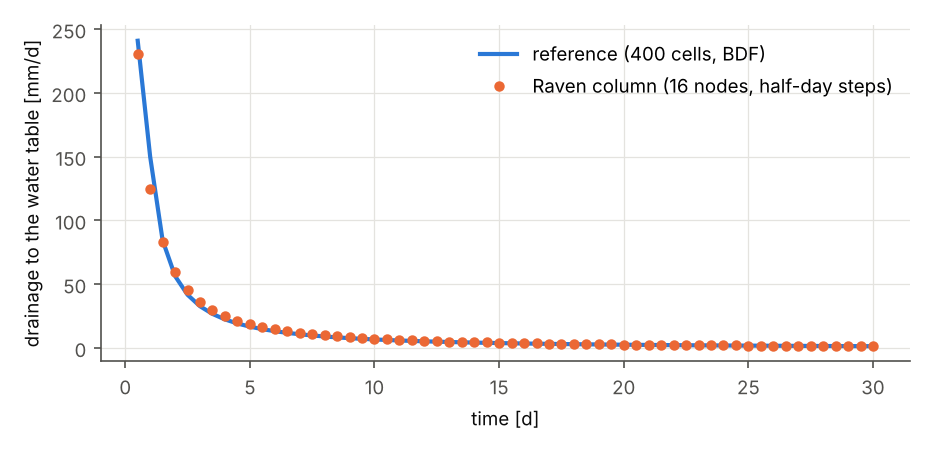
\includegraphics[width=0.49\linewidth]{figures/fig_sz_drainage.png}\hfill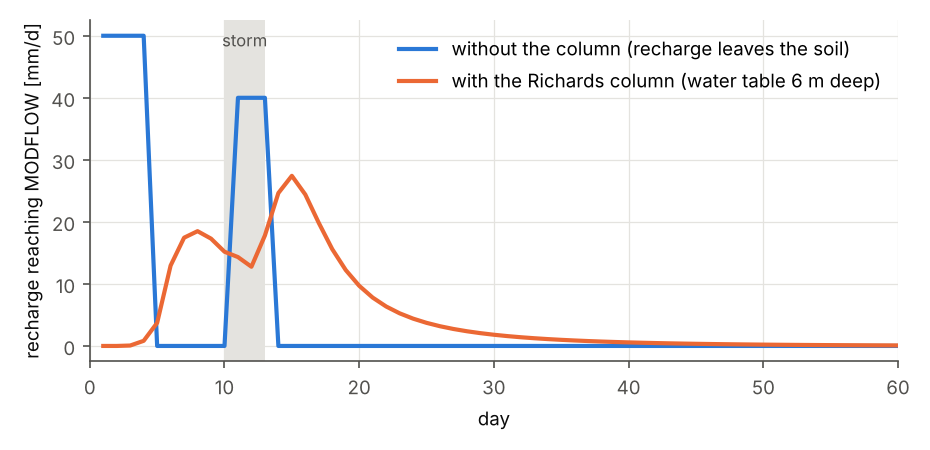
\includegraphics[width=0.49\linewidth]{figures/fig_sz_delay.png}
\caption{Left: drainage of a wet column to the water table, Raven's column against the reference solution
(step means). Right: recharge reaching MODFLOW after a 3-day storm with the water table 6~m deep
(test P1).}\label{fig:szdelay}\label{fig:szdrainage}
\end{figure}
\begin{figure}[!htbp]\centering
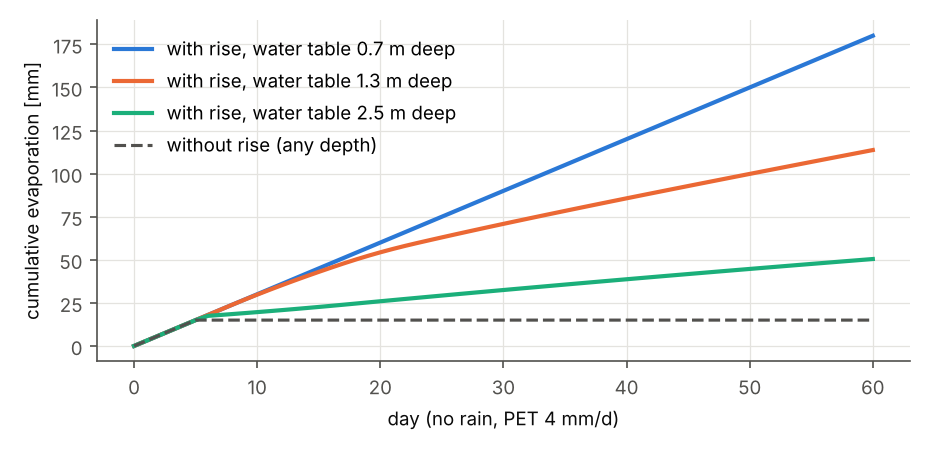
\includegraphics[width=0.49\linewidth]{figures/fig_sz_caprise.png}\hfill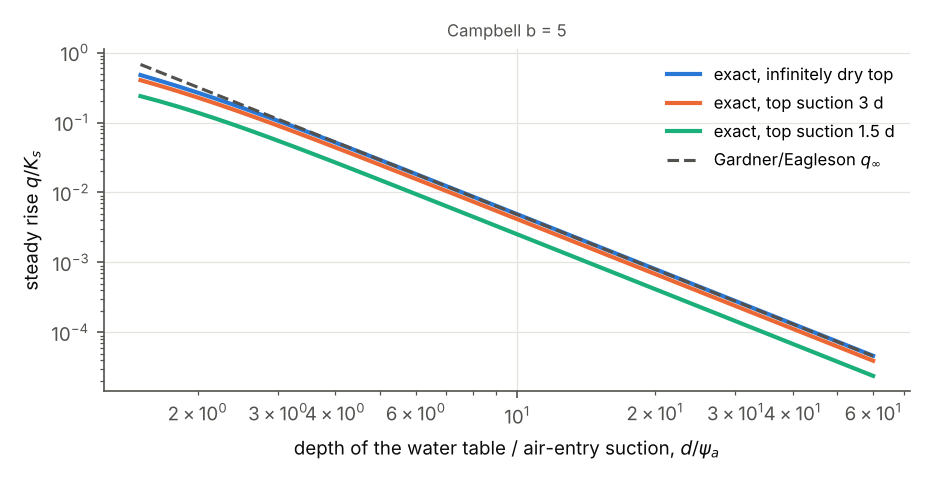
\includegraphics[width=0.49\linewidth]{figures/fig_sz_rise.png}
\caption{Left: evaporation from a drying soil over a shallow water table, with and without capillary rise (test P2).
Right: the steady rise from a water table (\ref{eq:rise}) for three suctions at the top, and Gardner's limit, which
overestimates the rise unless the soil is very dry.}\label{fig:szcaprise}\label{fig:szrise}
\end{figure}
\begin{figure}[!htbp]\centering
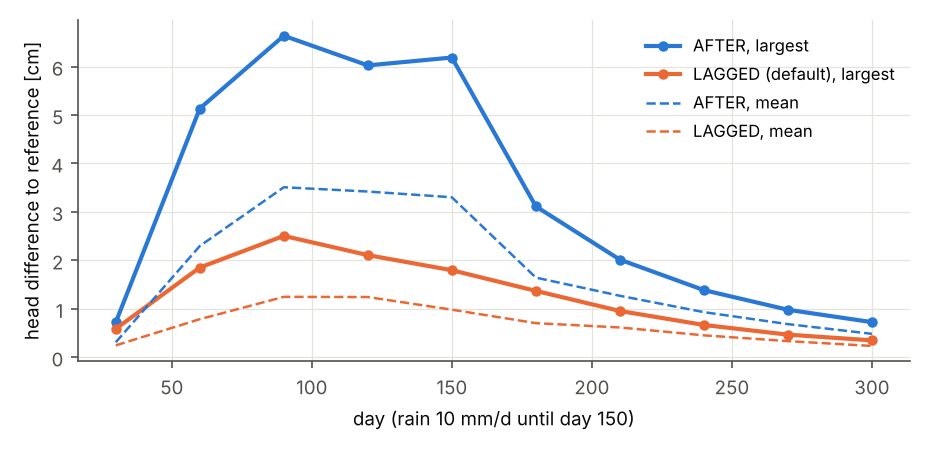
\includegraphics[width=0.56\linewidth]{figures/fig_sz_timing.png}\hfill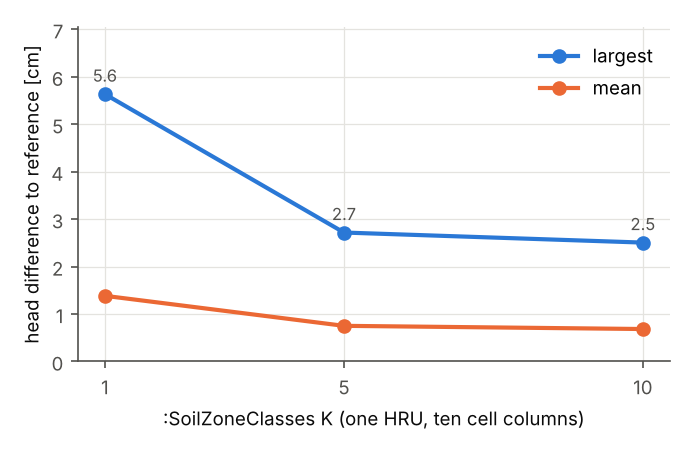
\includegraphics[width=0.42\linewidth]{figures/fig_sz_classes.png}
\caption{Left: head difference to the MODFLOW-only reference on the hillslope with the exchange after Raven's
processes (\cmd{AFTER}) and lagged (\cmd{LAGGED}, the default; test P5). Right: the same hillslope as one HRU, with Raven's
processes on 1, 5 and 10 classes of its columns (test P6).}\label{fig:sztiming}\label{fig:szclasses}
\end{figure}

\subsection{The interface iteration and MODFLOW's side}\label{sec:vszinterface}
Six scripts test the interface iteration, drained columns, heads far outside the model, negative recharge, MODFLOW's
budget as Raven books it and surface stores on soil-zone HRUs (Table~\ref{tab:vszinterface}; numbers of the quick mode, \cmd{RAVEN\_TEST\_QUICK=1}). The negative
recharge cases run in \cmd{test\_robustness.py} as R14--R22.
\begin{longtable}{P{0.13\linewidth}P{0.42\linewidth}P{0.36\linewidth}}
\caption{The interface and MODFLOW's side (\cmd{test\_interface\_stiff}, \cmd{test\_confined\_wet}, \cmd{test\_columns\_mf6},
\cmd{test\_robustness} R14--R22, \cmd{test\_mf6\_budget}, \cmd{test\_surface\_stores}).}\label{tab:vszinterface}\\
\toprule\hdr Test & Case & Result\\\midrule\endfirsthead
\caption[]{The interface and MODFLOW's side (continued).}\\
\toprule\hdr Test & Case & Result\\\midrule\endhead
S1 & low-$K_v$ top layer ($K_v$ 0.5~mm/d), wet spell from 3~m deep; columns from 1.5~m & every step converged; 4.0 (NONE) and 5.9 (RICHARDS) outer iterations per step; $F$ up to 1, column inflow 6\,530~m$^3$\\
S2 & $S_y$ 0.02, one base point per cell, rising water into a drying soil (kink drain) & converged; 4.4 / 6.0 outer iterations per step\\
S3 & explicit coupling over a 0.8~m top layer, egg-crate slope, specified head & no shortfall\\
S4 & \cmd{:SoilZoneIteration} 1 and 2 & 400 / 20 (NONE) and 400 / 60 (RICHARDS) supply-limited updates; largest take beyond the free water $2\cdot10^{-13}$~m$^3$/d\\
S5 & S4 with constant percolation and PET 5~mm/d from 1~m & take $2\cdot10^{-13}$~m$^3$/d\\
S6 & outer-iteration limit 1, iteration 0 and 1 & explicit; outputs identical\\
S7 & limits 2 and 3 & 6 of 10 steps converged (those without exchange); no ``no change \ldots to compare with''\\
S8 & connection test: stored case lowkv\_g57 without rain, $d_s$ 0.5~m, 16~m deep, head tolerance 0.05~m; default limit and limit 20 & 1 drop, its next update plain; with limit 20 the warning names the connection test at HRU 1, cell (1 1 6), fraction 0.0027 against 0\\
W1--W3 & confined layer below its bottom, generated and existing (ICELLTYPE from memory) & every step converged, no column kept wet\\
W5 & case Dc (existing, ICELLTYPE 1/0/1, ICONVERT 1, 20\,\% slope, dry then 30~mm/d) & 43 of 43 steps, 0 unconverged\\
W7 & confined model with a 10$^4$~m$^3$/d well, far heads that converge; W7c limit 3 & warned once; W7c completes, 8 MODFLOW-unconverged steps carried on, pumped head within 0.9\,\% of the default run, every warning's percentage equal to GWBudget's\\
W9, W10 & the same with limits 2 and 1 & stop: residual 2\,\% of the gross flow / the solve moved the head 1\,241~m; messages name head, cell (1 2 2), residual and causes\\
W12 & existing model with an inactive top layer, limit 2 & every interface warning names layer 2\\
W13 & the W7 model generated, \cmd{:SolverMaxOuterIterations 3} (steps 1--8 unconverged): restarts after unconverged steps & \cmd{:GWStartHeads} written after day 3 and carried unchanged through a restarted unconverged day, none after a converged day; a restart on day 4 equals the continuous run (difference 0)\\
M1--M4 & drained columns kept wet; a column delivers its inflow; \cmd{CONCEPTUAL} against a reference build; missing summary line & kept in 5 outer iterations; outflow 1.02 of the inflow; byte-identical except the balance-error \%\\
R14--R20 & negative recharge (\cmd{PERC\_GR4JEXCH}): split, cut by the top cell, hand-back, not held, existing model without \cmd{NEWTON} (confined variant), column upflow, sibling columns & identities at round-off; cut 437\,045~m$^3$; not held 3\,793 (LAGGED) / 2\,870 (AFTER)~m$^3$; not applied $-408\,000$~m$^3$, 0 with confined cells; not held only where the HRU's soil is empty (334~m$^3$)\\
R21 & a step with negative recharge in which wet unsaturated columns vanish under a water table raised by a specified head (\cmd{RICHARDS}; \cmd{KINEMATIC} in the full mode) & the vanished columns' water beyond $S_y\,\Delta h$ goes back to the soil zone as the link's rejected recharge; recharge identity 0\\
R22 & negative recharge with three depth classes, the hollow classes without a column (\cmd{RICHARDS}; \cmd{LAG} in the full mode) & MODFLOW's recharge on step 1 equals the top-cell limit (ratio 1.000000, as with one class); the cut, 2\,620~m$^3$, back to the soil zone\\
SW1--SW3 & \cmd{:SurfaceWaterExchange} on \cmd{DEPRESSION} of \cmd{:SoilZone PHYSICAL} HRUs, generated and existing model; a control with the water table above the ground at the outlet & stores' bed at the ground (model top + 1.0~m of soil zone); no discharge into the stores while every water table is below the ground; leakage 6\,135~m$^3$; existing model within $5\times10^{-6}$; control: discharge 1\,399~m$^3$\\
SW4 & restart of the control after 10 days, with a depression filled by groundwater to 64.6~mm (\cmd{DEP\_MAX} 50~mm) & the store is kept, not clipped to its maximum: Depression and the discharge into the stores equal the continuous run ($2.5\times10^{-9}$; a clip to the maximum would lose 583~m$^3$ and put the discharge 9\,\% off)\\
B1--B7 & steady existing model without STO (converged and OUTER\_MAXIMUM 3), gross flow, hourly dates, specified head under a dry cell, \cmd{:SoilZoneClasses 3}, audit guard counts & balance error $6\cdot10^{-12}$; residual equals the list file's IN$-$OUT within $1.3\cdot10^{-8}$ of the gross flow; gross flow equals TOTAL IN$+$TOTAL OUT within $5\cdot10^{-10}$; dates with times; warning names 2 columns over specified heads; no round-off as not held; guard counts 12 and 2\\
B8 & without \cmd{:SoilZone PHYSICAL}, \cmd{:SolverMaxOuterIterations} 2 (10 unconverged steps) and 1 (every step), and the Liard example (rivers and lakes) at 2: each row's residual over all its columns equals MODFLOW's negative residual on unconverged steps and 0 otherwise; run total ``discharge withheld''; at most ten warnings & step 1: 1\,039.4~m$^3$/d withheld = $-$balance error; run total 1\,062.5~m$^3$ = sum of rows; limit 1: 18\,511~m$^3$; 10 warnings (full mode)\\
B9 & \cmd{GWSoilExchange.csv} against \cmd{GWBudget.csv}: a generated model with an HRU wholly over specified-head cells, an existing model with a specified-head toe & on every date the four exchange columns summed over the HRUs equal \cmd{GWBudget.csv}'s within $2\cdot10^{-10}$ of the gross flow; the HRU over specified heads reports its base and water table\\\bottomrule
\end{longtable}
\noindent W4, W6 and W11 are reported as skipped: W4's rough-terrain cases run in \cmd{test\_rough\_terrain.py}; W6 (the
far-head warning once per ensemble member) and W11 (a head crossing the model) are not implemented as tests.

\subsection{Unsaturated-zone methods, depth classes and steady starts}\label{sec:vszmethods}
The \cmd{KINEMATIC} and \cmd{LAG} methods and the depth classes have their own tests, described with each method:
\cmd{test\_vz\_kinematic.py} K1--K9 (Section~\ref{sec:szvadosekw}), \cmd{test\_vz\_lag.py} LU, L1--L7, LS and the byte-identity
check LB (Section~\ref{sec:szvadoselag}), and \cmd{test\_vz\_classes.py} C1--C11 (Section~\ref{sec:vzclasses}). Among the
latter, C9 runs the rough-terrain case RT20 (stored existing model e43, \cmd{LAG}) with three depth classes through
\cmd{test\_rough\_terrain.py}: the saturated fraction stays within 0.0001 of the closure (limit 0.004) and no run fails; C10
writes a hotstart after a step that dropped a class column ($K=3$; after 4, 10 and 13 days): no mismatch warning, and the
restart within $7.5\times10^{-7}$ of the continuous run. \cmd{test\_vz\_initial.py} checks the steady start of
\cmd{:SoilZoneVadoseInitialFlux} (Section~\ref{sec:szvadose}):
\begin{itemize}
\item VI1, VI2, VI4: columns started at the steady profile carry their flux from the first step, with the storage at the start
in \cmd{GWModelSummary.txt}; hotstarts restore the columns; the columns' balance closes from step 1;
\item VI5: the steady start is for the flux each column receives, $(1-F)\,q$ (hummocks $\pm3$~m, water table 3~m deep,
$F=0.16$, 2~mm/d, \cmd{RICHARDS}, \cmd{KINEMATIC}, \cmd{LAG}, $K=1$ and 3): step-1 outflow = inflow = 100.8~m$^3$, 25.6~m$^3$
rejected;
\item VI6: a column that cannot carry $q$ (\cmd{K\_VERT} 1~mm/d under 2~mm/d) starts backed up: storage unchanged, outflow =
inflow = 40.000~m$^3$, 40.000 rejected, with a warning;
\item VI7: a restart with \cmd{:SoilZoneVadose NONE} from a file holding columns (\cmd{LAG}, $K=3$, negative recharge, 4 days):
a warning names the columns and their water, and \cmd{GWModelSummary.txt} reports it (248~m$^3$, the first run's final
unsaturated storage);
\item VI8: a restart with \cmd{:SoilZoneSubgrid 8} from a file written with 5 (\cmd{RICHARDS}, $K=3$): the columns' tops differ,
so they start at rest with a warning (0 against 5.37~m$^3$ written); with \cmd{:SoilZoneSubgrid 5} the written water is read exactly;
\item VI9: a restart with another method (the column case, $K=1$): written by \cmd{RICHARDS} and read by \cmd{KINEMATIC}, and
the other way round, the columns start at rest, the warning names the writing method and the run total reports the
first run's final storage (3.72 and 491~m$^3$; read as the other method's contents they would start with $+3\,669$ and
$-3\,628$~m$^3$); \cmd{RICHARDS} read by \cmd{LAG} starts with the written water;
\item VI10: a restart with a specified head added over HRU~1 (\cmd{LAG}, $K=1$, initial flux 30~mm/d): the 2 lines on its
cells are not used, and the warning and the run total give their 77.5~m$^3$ (start storage plus that volume equals the
file's water);
\item VI11: a generated model whose \cmd{:BoundaryHead} series holds the outlet cells at the start builds no column on them
(start storage 839.0~m$^3$, as with a fixed head; built there, the columns would ship 120~m$^3$ of initial-flux water to
the specified heads in step 1);
\item VI12: columns over an existing model's own specified heads (\cmd{KINEMATIC}, $K=3$, periods 3--5): a restart on day 4
rebuilds them at rest and ends them again, but only columns that held water are counted, so the two parts' run totals
add up to the continuous run's (18 columns, 225.75~m$^3$);
\item VI13: a generated model's \cmd{:BoundaryHead} series below the aquifer on days 1--3 (columns form on its cells) and
near the ground from day 4, restarted from day 3's \cmd{solution.rvc} (\cmd{LAG}, $K=1$; \cmd{KINEMATIC}, $K=3$,
\cmd{LAGGED}): the restart builds those columns from the file and ends them in its first step, so \cmd{GWBudget.csv} from
day 4 equals the continuous run's (deviation 0; day 4's recharge onto the specified heads 51.79 and 94.32~m$^3$/d).
\end{itemize}

\subsection{Input handling}\label{sec:vszinputs}
\begin{longtable}{P{0.07\linewidth}P{0.55\linewidth}P{0.30\linewidth}}
\caption{Soil zone and hotstarts: input handling (\cmd{test\_inputs.py}; short runs of the CT1 column unless stated).}\label{tab:vszinputs}\\
\toprule\hdr Test & Case & Result\\\midrule\endfirsthead
\caption[]{Soil zone and hotstarts: input handling (continued).}\\
\toprule\hdr Test & Case & Result\\\midrule\endhead
I1 & \cmd{HYDRAUL\_COND} missing for the soil class of the bottom soil-zone layer & stops (``needs HYDRAUL\_COND'')\\
I2 & \cmd{:SoilZoneIteration} with the update count only (0) & accepted; explicit, no interface update\\
I3 & \cmd{:SoilZone PHYSICAL} followed by \cmd{:SoilZone CONCEPTUAL} & the last counts: a conceptual run\\
I4 & soil-zone options under \cmd{CONCEPTUAL} & reported as ignored\\
I5 & a \cmd{:GWSoilZoneColumns} block with a column missing & reported (``do not match its soil-zone columns'')\\
I6 & the same block with its rows in another order & used (matched by cell)\\
I7 & groundwater blocks in the \cmd{.rvc} of a run without \cmd{:GroundwaterModel} & skipped; Raven's initial conditions after them apply\\
I8 & \cmd{:SurfaceWaterExchange} on a soil-zone layer & refused\\
I9 & a damaged \cmd{:GWHeads} header (\cmd{-1 2 2}; \cmd{100000 100000 100000}) & stops with a message\\
I10 & \cmd{:StartTime} in the \cmd{.rvc}, run under valgrind & no uninitialised read in \cmd{ParseInitialConditionsFile} or \cmd{TimeDifference}\\
I11 & \cmd{:BoundaryHead NOPE} beside boundary \cmd{EDGE}; \cmd{:WellFlowRate 7} with only well 1 & stop naming the series and the boundaries or wells there are; the right names run\\
I12 & \cmd{:SeepageToRaven}, \cmd{:KeepPackages}, \cmd{:MF6StartDate}, \cmd{:MF6Model} on a model Raven builds; depth classes and initial flux with \cmd{NONE}; \cmd{:SoilZoneAquiferClass} on a generated model; an unknown profile attribute; \cmd{LAYERS BOTTOM} & the four stop; the next three are reported as ignored; the last two stop\\
I13 & a missing \cmd{.rvg} file; a short \cmd{:Wells} row & named in \cmd{Raven\_errors.txt}; the message names \cmd{:Wells}\\
I14 & age tracer (no groundwater): 20 days against 7 + 7 + 6 days chained through \cmd{solution.rvc} & ages of every store and the outflow within $2\times10^{-4}$~d plus $10^{-5}$ of the age (the six digits of \cmd{Ages.csv}) of the continuous run, largest difference $10^{-4}$~d; \cmd{:StartTime} the start of each part, \cmd{:AgeTracerDatum} 2000-01-01 in the restarted parts\\
I15 & age-tracer chains across year boundaries: 1999-12-25 (7 + 7 + 6 days), 1998-12-20 (400 + 380 days; quick mode 12 + 400 + 8) & every part runs; ages within the limit of I14, largest difference $10^{-4}$~d; \cmd{:AgeTracerDatum} 1999-12-25 and 1998-12-20\\
I16 & age tracer started from the \cmd{solution.rvc} of a 30-day spin-up without it & ages 0 at the start, 1~d after the first day; no \cmd{:AgeTracerDatum}\\
I17 & EnKF, 3 members, one well, \cmd{:ExtraRVTFilename} with $-100$, $-200$, $-300$~m$^3$/d & each member pumps its own rate; a series naming no well stops the run\\
I17b & EnKF, 2 members whose \cmd{:ExtraRVTFilename} gives a \cmd{:BoundaryHead} series (99~m, then 70~m below the aquifer) to a specified head the base \cmd{.rvt} leaves fixed & each member's model is built with its series: the cells are released on days 3--6, nothing is booked onto them, and both members' \cmd{GWBudget.csv} equal the single run with the series in its \cmd{.rvt}\\
I18 & \cmd{:GWSoilZoneColumns} with \cmd{nan} or $-50$~mm, \cmd{:GWHeads} with \cmd{nan} & each stops with a message naming the block; the undamaged file runs\\
I19 & \cmd{:Transport Nitrate} (\cmd{CONCEPTUAL}, \cmd{PHYSICAL}) and \cmd{:Transport AGE} with \cmd{:GroundwaterModel MODFLOW6}; the same model without groundwater & the coupled runs stop naming the constituent; the run without groundwater completes\\
I20 & a specified head with \cmd{HEAD} 0 (below every cell) and a \cmd{:BoundaryHead} series of 99.5~m; the same without the series & placed by the series: 2 cells, flow 1\,390~m$^3$; without it no cell and a warning naming the boundary, its head and the highest cell bottom\\
I21 & head boundary \cmd{EDGE} (\cmd{HEAD} 90) with a series of 99~m on day 1, then 90~m; layer 1 from 100 to 97~m: (a) a GHB (\cmd{LAYERS TOP}) against an aquifer at 95~m; (b) a CHD (\cmd{LAYERS TOP}); (c) a CHD (\cmd{LAYERS ALL}, 99~m for 3 days), restarted on day 4 & (a) the GHB drains on days 2--6 ($-7\,915$ to $-2\,275$~m$^3$/d), as with \cmd{HEAD} 90 alone; a series of 90~m gives the outputs of \cmd{HEAD} 90; (b) the water table falls below 97~m (93.8 to 92.9~m): no cell is held at the bottom of layer 1; (c) the restarted run has the same 4 CHD cells and the same flows and heads as the continuous run\\
I21 (d) & a column with no cell held: 8 HRUs, the last wholly on \cmd{EDGE} (\cmd{LAYERS ALL}), rain 20~mm/d, a series of 99~m on days 1--2 and 70~m (below the aquifer) on days 3--6; \cmd{CONCEPTUAL} and \cmd{PHYSICAL} & days 3--6: CHD flow 0 and nothing booked onto specified-head cells; MODFLOW's recharge equals Raven's (\cmd{CONCEPTUAL}); the column's soil-zone link exchanges 425 to 42~m$^3$/d with the aquifer (\cmd{PHYSICAL}); every identity holds\\
I21 (e) & \cmd{LAYERS TOP}, \cmd{HEAD} 90 and a series of 99~m on every day, CHD and GHB & the cells of layer 1 only (2), none switched off\\
I21 (f) & a steady-state first period at 90~m (series 90, 99, 99, 90, 90, 99~m) & the run total counts the steady period's 2 cells: 8 cell-steps against 6 without it\\
I22 & \cmd{:InitialGWHeads ELEVATION 98,5}, \cmd{H98.5}, \cmd{0x62}, \cmd{98.5}, \cmd{98.5\# note} and \cmd{98.5 \# note}; \cmd{:InitialGWHeads FROM\_PROFILE 0}; a \cmd{:GWHeads} value \cmd{98.1x} & the first three stop naming the command and the token (surplus value '5'; not a number), the next three start at 98.5~m; \cmd{FROM\_PROFILE 0} stops (takes no value); the damaged value stops naming the block\\
I23 & two \cmd{:SpecifiedHeadBoundary} commands on the same file (\cmd{HEAD} 99 and 99.5); two \cmd{:GeneralHeadBoundary} commands on it & the first stops before MODFLOW starts, naming both boundaries and the cell; the second runs\\\bottomrule
\end{longtable}

\subsection{Robustness}\label{sec:vszrobust}
\begin{longtable}{P{0.07\linewidth}P{0.55\linewidth}P{0.30\linewidth}}
\caption{Soil zone: robustness (\cmd{test\_robustness.py}; hard cases of the interface). R14--R22, the negative-recharge
cases, are in Table~\ref{tab:vszinterface}.}\label{tab:vszrobust}\\
\toprule\hdr Test & Case & Result\\\midrule\endfirsthead
\caption[]{Soil zone: robustness (continued).}\\
\toprule\hdr Test & Case & Result\\\midrule\endhead
R1 & stiff flat column: drainable porosity 0.02 against $S_y=0.25$, high conductance & every step converged; at most 12 updates, 27 outer iterations\\
R2, R2c & one HRU over ten cells against ten one-cell HRUs; R2c with constant-rate percolation & outflow $-0.2\,\%$, MODFLOW recharge ratio 1.00; R2c outflow $-0.2\,\%$\\
R3 & \cmd{RECHARGE\_DELAY} with \cmd{:SoilZone PHYSICAL} & refused\\
R4 & a smoothing depth below 0.1~m & warned\\
R5 & hourly steps, smoothing depth 0.001~m & no unconverged step; MODFLOW error $1.1\times10^{-11}$\\
R6 & slope 0.1 with $5\times5$ DEM points per cell & converged; at most 8 updates\\
R7 & explicit mode (\cmd{:SoilZoneIteration 0}) & no shortfall\\
R8 & one column $10^{-6}$~mm wetter than the others & heads stay uniform ($3.7\times10^{-9}$~m)\\
R9 & hotstart columns that cannot hold the \cmd{.rvc} layer split & 4\,000~m$^3$ redistribution reported in step 1, 0 later\\
R10 & water rising into a thin soil on a steep, low-storage slope, update budget 1 and explicit mode & no shortfall\\
R11 & explicit mode on the R2 hillslope against the iterated run & outflow within 0.6\,\%\\
R12 & explicit mode, 15 outer iterations, water rising into cells dry at the head of linearization & converged; outflow within 0.6\,\%; MODFLOW error $10^{-7}$\\
R13 & stiff low-storage slope, budget 1, 12 outer iterations, MODFLOW unconverged & neither residual nor shortfall handed to Raven: outflow 1.01 times the iterated run's\\
R15b & a negative-recharge cut on a draining soil zone: 8.67~mm cut while the wet soil drains & soil zone after step 1 at least its field-capacity water (126.08 against 120~mm)\\\bottomrule
\end{longtable}
